\let\negmedspace\undefined
\let\negthickspace\undefined
\documentclass[journal]{IEEEtran}
\usepackage[a5paper, margin=10mm, onecolumn]{geometry}
%\usepackage{lmodern} % Ensure lmodern is loaded for pdflatex
\usepackage{tfrupee} % Include tfrupee package

\setlength{\headheight}{1cm} % Set the height of the header box
\setlength{\headsep}{0mm}     % Set the distance between the header box and the top of the text

\usepackage{gvv-book}
\usepackage{gvv}
\usepackage{cite}
\usepackage{amsmath,amssymb,amsfonts,amsthm}
\usepackage{algorithmic}
\usepackage{graphicx}
\usepackage{textcomp}
\usepackage{xcolor}
\usepackage{txfonts}
\usepackage{listings}
\usepackage{enumitem}
\usepackage{mathtools}
\usepackage{gensymb}
\usepackage{comment}
\usepackage[breaklinks=true]{hyperref}
\usepackage{tkz-euclide} 
\usepackage{listings}
% \usepackage{gvv}                                        
\def\inputGnumericTable{}                                 
\usepackage[latin1]{inputenc}                                
\usepackage{color}                                            
\usepackage{array}                                            
\usepackage{longtable}                                       
\usepackage{calc}                                             
\usepackage{multirow}                                         
\usepackage{hhline}                                           
\usepackage{ifthen}                                           
\usepackage{lscape}
\begin{document}

\bibliographystyle{IEEEtran}
\vspace{3cm}

\title{2.4.23}
\author{EE25btech11028 - J.Navya sri}
% \maketitle
% \newpage
% \bigskip
{\let\newpage\relax\maketitle}




\textbf{Question:}\\

Do the points \( (3, 2) \), \( (-2, -3) \), and \( (2, 3) \) form a triangle? If so, name the type of triangle formed.

\vspace{0.5cm}
\textbf{Solution:} 
Let the position vectors of the points be:
\[
\vec{A} = (3, 2), \quad \vec{B} = (-2, -3), \quad \vec{C} = (2, 3)
\]

\subsection*{Step 1: Check if the points are collinear}

Calculate area of the triangle using vector cross product magnitude:

\begin{equation}
\text{Area} = \frac{1}{2} \left| (\vec{B} - \vec{A}) \times (\vec{C} - \vec{A}) \right| \tag{1}
\end{equation}

Compute vectors:

\[
\vec{B} - \vec{A} = (-2 - 3,\, -3 - 2) = (-5, -5) \tag{2}
\]
\[
\vec{C} - \vec{A} = (2 - 3,\, 3 - 2) = (-1, 1) \tag{3}
\]

Calculate the 2D cross product magnitude:

\begin{align}
|(\vec{B} - \vec{A}) \times (\vec{C} - \vec{A})| &= |(-5)(1) - (-5)(-1)| \notag \\
&= |-5 - 5| = 10 \tag{4}
\end{align}

Therefore,

\[
\text{Area} = \frac{1}{2} \times 10 = 5 \neq 0 \tag{5}
\]

Since area \(\neq 0\), points are not collinear and hence form a triangle.



  \subsection*{Step 2: Calculate the side lengths}

Length of side \(AB\):

\begin{equation}
|\vec{B} - \vec{A}| = \sqrt{(-5)^2 + (-5)^2} = \sqrt{50} \tag{6}
\end{equation}

Length of side \(BC\):

\begin{equation}
|\vec{C} - \vec{B}| = \sqrt{(2 + 2)^2 + (3 + 3)^2} = \sqrt{16 + 36} = \sqrt{52} \tag{7}
\end{equation}

Length of side \(AC\):

\begin{equation}
|\vec{C} - \vec{A}| = \sqrt{(-1)^2 + 1^2} = \sqrt{2} \tag{8}
\end{equation}



\subsection*{Step 3: Determine the type of triangle}

Since

\[
\sqrt{50} \neq \sqrt{52} \neq \sqrt{2}
\]

all sides are unequal.

\section*{Final Answer}

\[
\boxed{
\text{Yes, the points form a scalene triangle.}
}
\]


\textbf{Graphical Representation:}

\begin{center}
\begin{tikzpicture}[scale=0.8]
    % Draw axes
    \draw[->] (-5,0) -- (5,0) node[right] {x};
    \draw[->] (0,-5) -- (0,5) node[above] {y};

    % Grid (optional)
    \draw[step=1cm,gray!30,very thin] (-5,-5) grid (5,5);

    % Points
    \coordinate (A) at (3,2);
    \coordinate (B) at (-2,-3);
    \coordinate (C) at (2,3);

    % Draw triangle
    \draw[thick, blue] (A) -- (B) -- (C) -- cycle;

    % Draw and label points
    \filldraw[black] (A) circle (2pt) node[anchor=west] {A(3,2)};
    \filldraw[black] (B) circle (2pt) node[anchor=east] {B(-2,-3)};
    \filldraw[black] (C) circle (2pt) node[anchor=west] {C(2,3)};
    \end{tikzpicture}
    
        % Add "Fig. 0" text below the figure
    \vspace{0.5cm} % space between figure and text
    \textbf{Fig. 0}

\end{center}

\end{document}

